\section{Speed Measurements} \label{sec:measurements-speed}
This section shows the result of two speed comparisons and discusses the conclusions that were drawn. The shown measurements are always the mean of at least ten results. A table showing all exact results was added to the appendix.

The measuring was done by inserting profiling code. The .Net Framework provides helpful tools for such measurements, so the actually added code was only a few lines long.

%TODO: Used environment
%TODO: Add table of results (and link it here)
%TODO: Add glossary entry for '.Net Framework', 'CPlan', 'K-Means'
%TODO: K-Means with features!

\subsection{K-Means}
Figure \ref{fig:kmeans_speed} shows speed measurements of the K-Means algorithm applied to Weimar in different settings.

The used parameters were for all four measurement categories the following (Those parameters can be manually set as shown in the appendix in figure \ref{fig:applied_k-means_GUI}.):

\begin{itemize}
    \item No live visualisation
    \item Number of tries: 10
    \item Iterations per try: 10
    \item Minimal cluster count: 5
    \item Maximal cluster count: 15
\end{itemize}

The different bars of the diagram have the following meaning:

\begin{itemize}
    \item \textbf{Original:} Initial implementation of K-Means without performance or other improvements.
    \item \textbf{Original \& Shortest Path:} Implementation of K-Means without performance improvement but additional run of \acrshort{APSP} (Dijkstra, not parallel) to improve the result quality.
    \item \textbf{Parallel:} Implementation of K-Means which runs multiple tries parallelised.
    \item \textbf{Parallel \& Shortest Path:} Implementation of K-Means which runs multiple tries parallelised and additionally runs \acrshort{APSP} (Dijkstra, parallel).
\end{itemize}

\begin{figure}[!ht]
    \centering
    \begin{mdframed}[style=mdthight]
        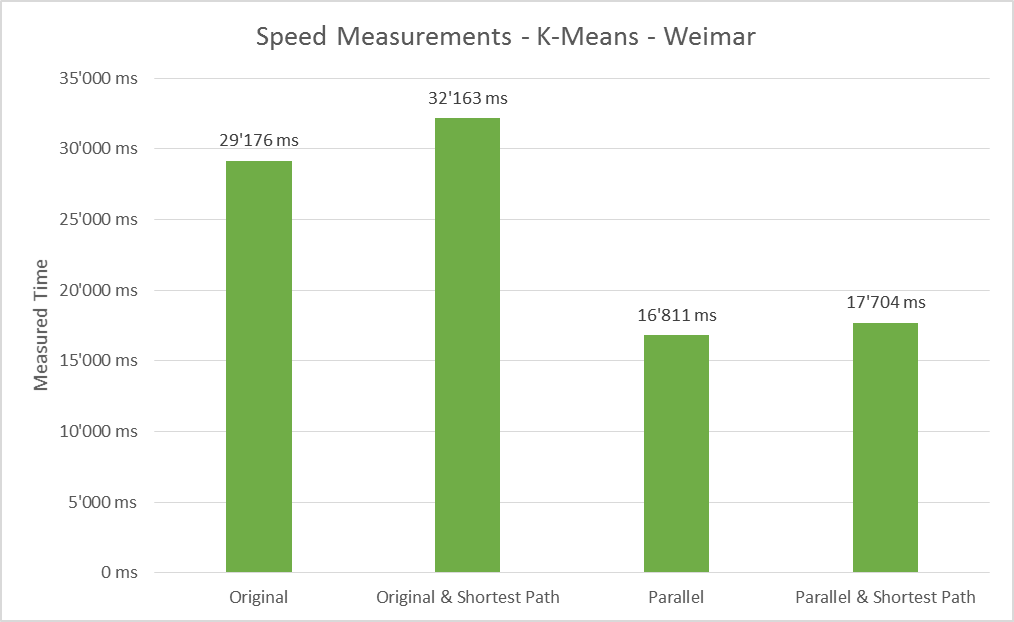
\includegraphics[width=\textwidth]{kmeans_speed.png}
    \end{mdframed}
    \caption{Speed measurements of the K-Means clustering algorithm applied to Weimar \label{fig:kmeans_speed}}
\end{figure}

As it is clearly visible, parallelisation almost doubles the performance of K-Means. Adding an \acrshort{APSP} does only inflict a minor slowdown in both the parallel and the original implementation.

\subsection{Hierarchical Clustering}
Figure \ref{fig:hierarchical_clustering_speed} shows speed measurements of hierarchical clustering algorithms applied to Weimar.

The used parameters were for all measurements the following (Those parameters can be manually set as shown in the appendix in figure \ref{fig:applied_HC_clustering_GUI}.):

\begin{itemize}
    \item Show slider dialog (figure \ref{fig:applied_HC_clustering_slider_GUI}): no
    \item Number of clusters: 10
    \item Modify Output \ref{sec:outout_modification}: yes
\end{itemize}

The different bars show the speed measurements of the implemented variations of hierarchical clustering algorithms. Each algorithm was measured in conjunction with different \acrshort{APSP} algorithms. The following hierarchical clustering implementations were measured:

\begin{itemize}
    \item \textbf{UPGMA (without distance caching):} Hierarchical clustering using the \acrshort{UPGMA} reduction formula, without using cluster distance caching. Distances between clusters were calculated every time they were needed.
    \item \textbf{UPGMA (fast / cached distances):} Hierarchical clustering using the \acrshort{UPGMA} reduction formula. Different than the previous, here distance caching \ref{sec:concept_distance_caching} was applied.
    \item \textbf{WPGMA (fast / cached distances):} Same clustering as the previous, but using the \acrshort{WPGMA} reduction formula.
\end{itemize}

The following \acrshort{APSP} algorithms were measured:

\begin{itemize}
    \item \textbf{Floyd-Warshall:} Regular Floyd-Warshall algorithm.
    \item \textbf{Dijkstra:} Regular \acrshort{SSSP} Dijkstra algorithm started from each vertex separately to create an \acrshort{APSP} algorithm. See \ref{sec:shortest_path} for more details.
    \item \textbf{Dijkstra Parallel:} The same as the previous with the difference that all Dijkstra algorithm runs are executed parallelised.
\end{itemize}

\begin{figure}[!ht]
    \centering
    \begin{mdframed}[style=mdthight]
        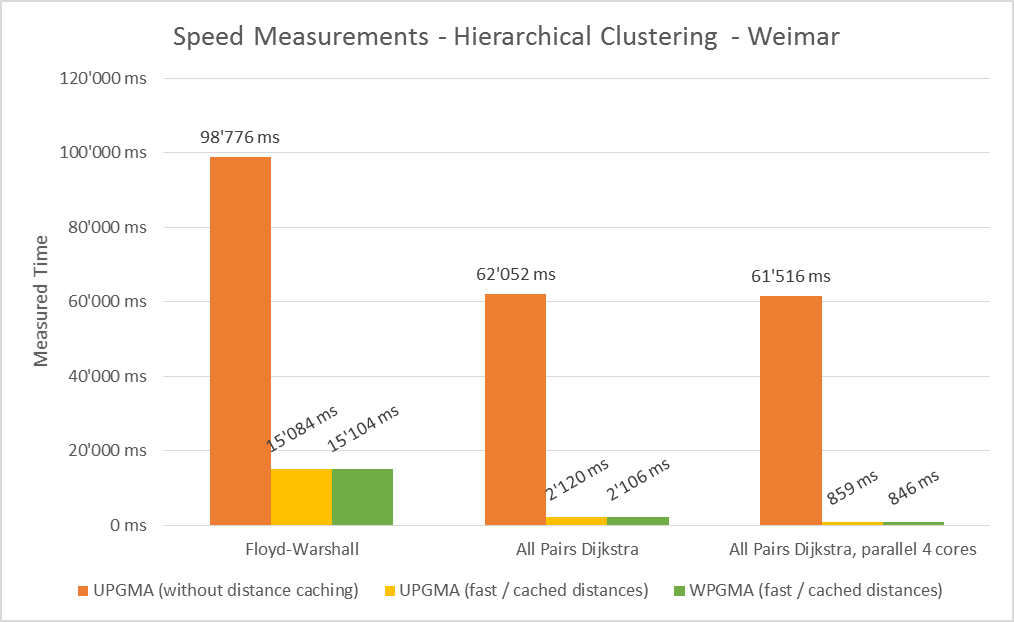
\includegraphics[width=\textwidth]{hierarchical_clustering_speed.png}
    \end{mdframed}
    \caption{Speed measurements of hierarchical clustering applied to Weimar \label{fig:hierarchical_clustering_speed}}
\end{figure}

The caching of cluster distances resulted in a significant speed improvement over the non-cached variation as it was expected. When comparing the speed of the applied \acrshort{APSP} algorithms, the parallelised Dijkstra solution performed the best. The parallelisation lead to more than double the speed of clustering with WPGMA over the non-parallel version. Both versions of the Dijkstra algorithm far outperformed the Floyd-Warshall algorithm in any of the measured hierarchical clustering variations.

\pagebreak
\section{Cluster Analysis}
\label{sec:measurements-cluster-analysis}
In this section the provided measurement methods \ref{sec:clusterRating} are used to compare the measured results between the different districts/areas. The following images were generated with the cluster algorithm FastUPGMA \ref{sec:UPGMAandWPGMA} on Weimar with \textit{Modified Output} and \textit{Number of Clusters} count 16.

A example for every district from the section \ref{sec:concept_cluster_analysis} was found. Three different colours can be observed. Red labelled edges are within the cluster. Grey edges are transitions between different clusters and black edges are outside of the cluster.

As expected in section \ref{sec:historyDistinct} the historic subgraph (figure \ref{fig:result_historic_district}) had a high block count on a small area. The street count, the vertex connections mean and the density are high. All results for this cluster can be viewed in table \ref{tab:measured_cluster_ratings} cluster number C1.

\begin{figure}[ht]
    \centering
    \begin{mdframed}[style=mdthight, userdefinedwidth=0.4\textwidth, align=center]
        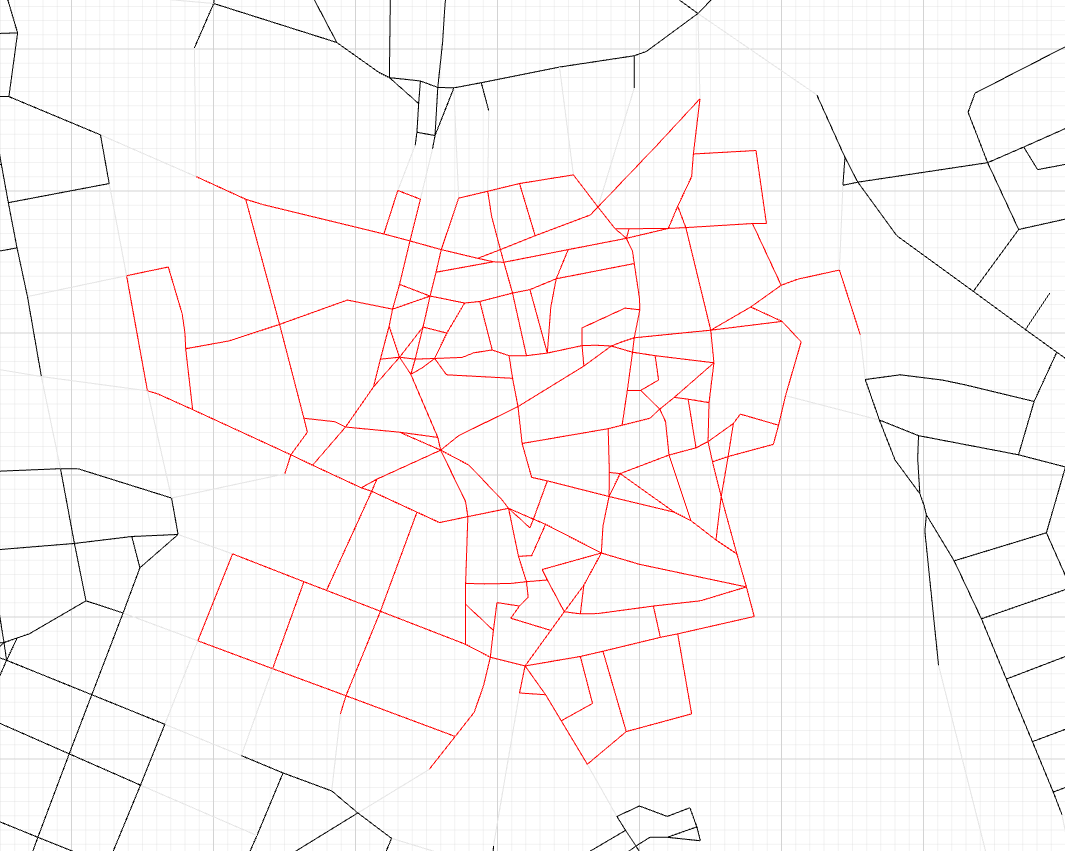
\includegraphics[width=\linewidth]{district_result_historic.png}
    \end{mdframed}
    \caption{Historic District Subgraph}
    \label{fig:result_historic_district}
\end{figure}
\FloatBarrier

Like anticipated in section \ref{sec:businessDistinct} the business district (figure \ref{fig:result_business_district}) had the highest relative block area (A/Ac) and a very high integration value. The mean connection count and the density are much higher compared with the historic district. This insights can be observed in table \ref{tab:measured_cluster_ratings} cluster number C2.

\begin{figure}[ht]
    \centering
    \begin{mdframed}[style=mdthight, userdefinedwidth=0.4\textwidth, align=center]
        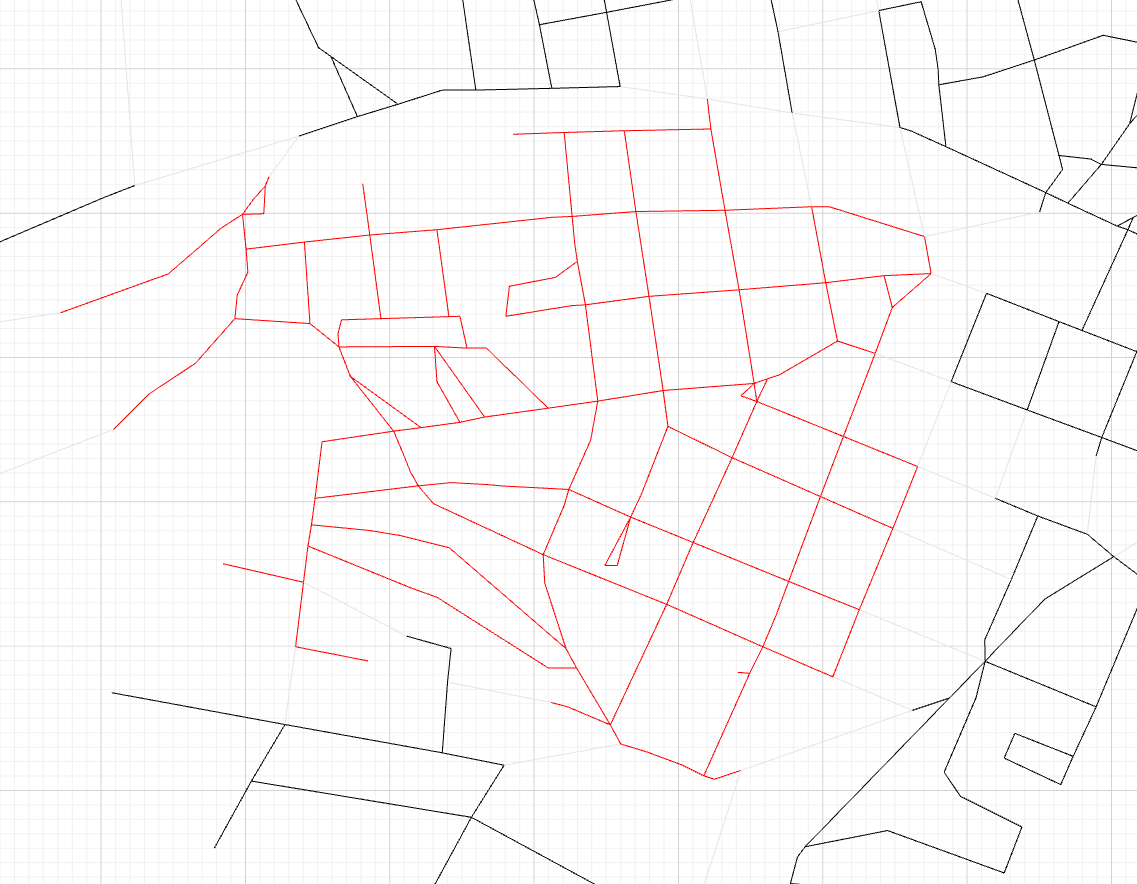
\includegraphics[width=\linewidth]{district_result_business.png}
    \end{mdframed}
    \caption{Business District Subgraph}
    \label{fig:result_business_district}
\end{figure}
\FloatBarrier

A detected outskirts subgraph can be viewed in figure \ref{fig:result_outskirts_district}. The measured results can be found in table \ref{tab:measured_cluster_ratings} cluster number C3. They show as expected a high street length variance and median. The density is very high because of a low street count on a big area.

\begin{figure}[ht]
    \centering
    \begin{mdframed}[style=mdthight, userdefinedwidth=0.6\textwidth, align=center]
        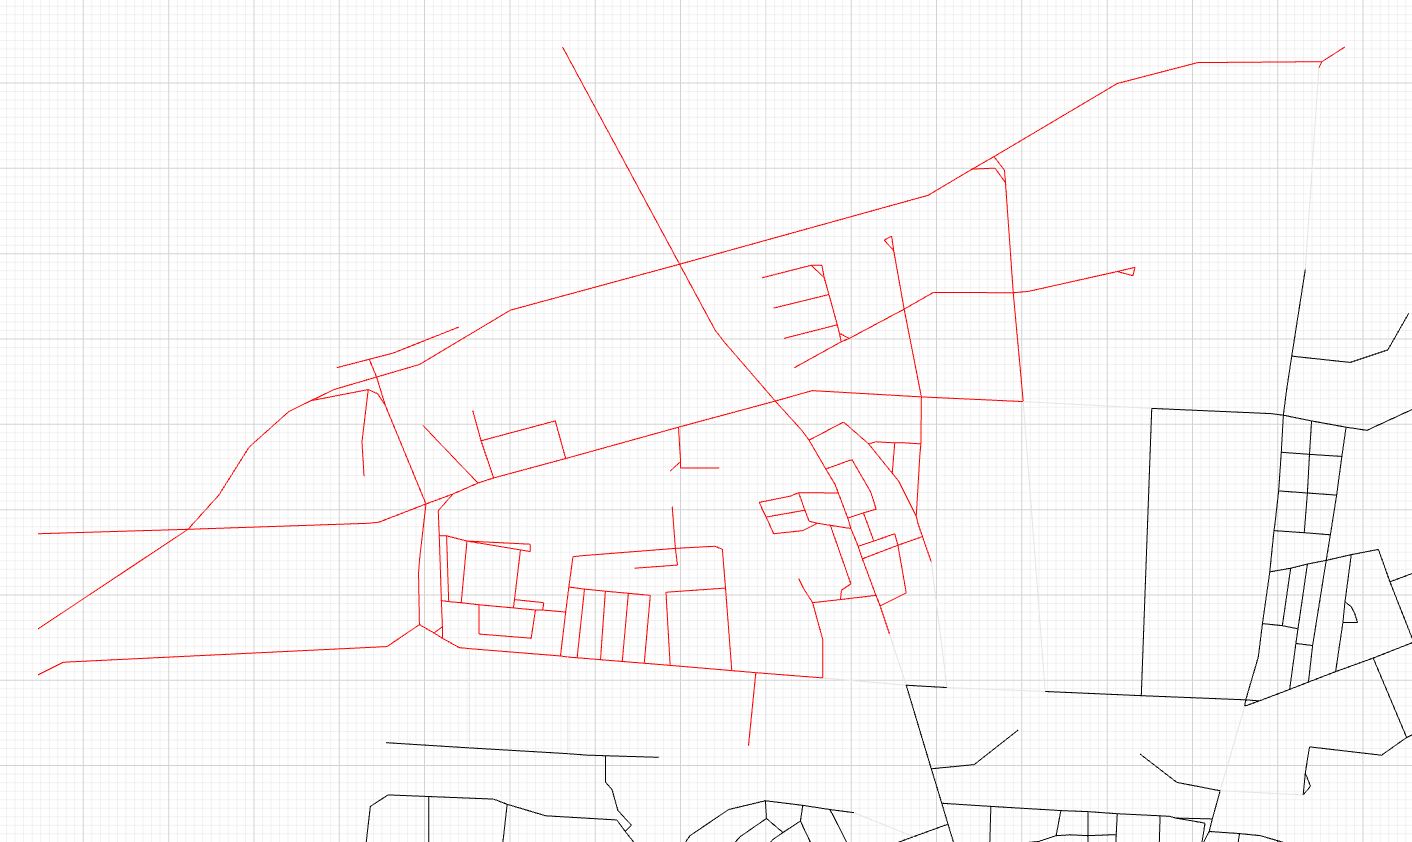
\includegraphics[width=\linewidth]{district_result_outskirts.png}
    \end{mdframed}
    \caption{Outskirts Subgraph}
    \label{fig:result_outskirts_district}
\end{figure}
\FloatBarrier

\FloatBarrier
\subsection{Measured Data}
\label{sec:ClusterAnalysisMeasurements}
The following table \ref{tab:cluterAnalysisDescription} contains the parameters with additional descriptions. Of every parameter the minimal (min), maximal (max), mean (average) and the median value can be calculated. Because the min, max values don't have any relevance they were skipped in this table. All measurements can be observed in the appendix in \ref{sec:measurements_full_table}.

\begin{table}[!ht]
\centering
\begin{tabular}{ | l | l |} \hline
    \textbf{Parameter} & \textbf{Description} \\
    \hline

    Total Area &  Area of the convex hull \\
    Total Length & Sum of the street length \\
    Density & 'Total Area' divided by 'Total Length' \\
    \hline

    Street Length Min/Max/Mean & Shortest/Longest/Average street length  \\
    Street Length Median & Middle value of the length dataset \\
    Street Length Variance & Sigma of the normal distribution curve of the variance \\
    \hline

    Vertex Connections & Mean connected edges per vertex  \\
    \hline

    Street Angle Min/Max/Mean & Smallest/Biggest/Average angle between two edges \\
    Street Angle Variance & Sigma of the normal distribution curve of the angles \\
    \hline

    Block Count & Total number of blocks \\
    Block Area Min/Max/Mean & Shortest/Biggest/Average block area \\
    Block Area A/Ac Min/Max/Mean & Block area divided to a minimal circle around a block \\
    \hline

    Integration Min/Max/Mean & Normalised In-Centrality \\
    \hline

    Choice Min/Max/Mean & Normalised In-Betweenness-Centrality \\
    \hline
\end{tabular}
\caption{Parameter with descriptions for table \ref{tab:measured_cluster_ratings}}
\label{tab:cluterAnalysisDescription}
\bigskip
\bigskip
\centering
\begin{tabular}{ | l | l | l | l | l | } \hline
    \textbf{Parmater} &
    & \textbf{C1} \ref{sec:historyDistinct}
    & \textbf{C2} \ref{sec:businessDistinct}
    & \textbf{C3} \ref{sec:outskits}  \\
    \hline

    \multirow{2}{*}{Total}
    & Area & 1838.05 & 1956.59 & 7802.74 \\
    & Length & 806.92 & 643.50 & 1069.81 \\
    \hline

    & Density & 2.28 & 3.04 & 7.29 \\
    \hline

    \multirow{3}{*}{Street Length}
    & Mean & 2.72 & 3.85 & 4.82 \\
    & Median & 2.30 & 3.65 & 3.28 \\
    & Variance & 1.70 & 2.19 & 5.00 \\
    \hline

    Vertex
    & Connections & 3.04 & 2.84 & 2.45 \\
    \hline

    \multirow{2}{*}{Street Angle}
    & Mean & 119.03 & 123.75 & 137.18 \\
    & Variance & 124.68 & 131.65 & 129.47 \\
    \hline

    \multirow{3}{*}{Block}
    & Count & 55 & 35 & 26 \\
    & Area Mean & 6.54 & 13.65 & 76.30 \\
    & A/Ac Mean & 0.18 & 0.23 & 0.18 \\
    \hline

    Integration
    & Mean & 0.49 & 0.59 & 0.78 \\
    \hline

    Choice
    & Mean & 0.10 & 0.05 & 0.04 \\
    \hline
\end{tabular}
\caption{Measured results from Historic District (C1) \ref{sec:historyDistinct}, Business District (C2) \ref{sec:businessDistinct} and Outskirts Area (C3) \ref{sec:outskits}}
\label{tab:measured_cluster_ratings}

\end{table}
